\vspace{-5pt}
\section{Qualitative results for vision and language tasks}\label{sec:sup_experiments}

In this section we provide more qualitative results for \gcam{} and \cgb{} applied to the task of image classification, image captioning and VQA.
\vspace{-5pt}
\subsection*{1. Image Classification}

\begin{figure*}
 \centering
 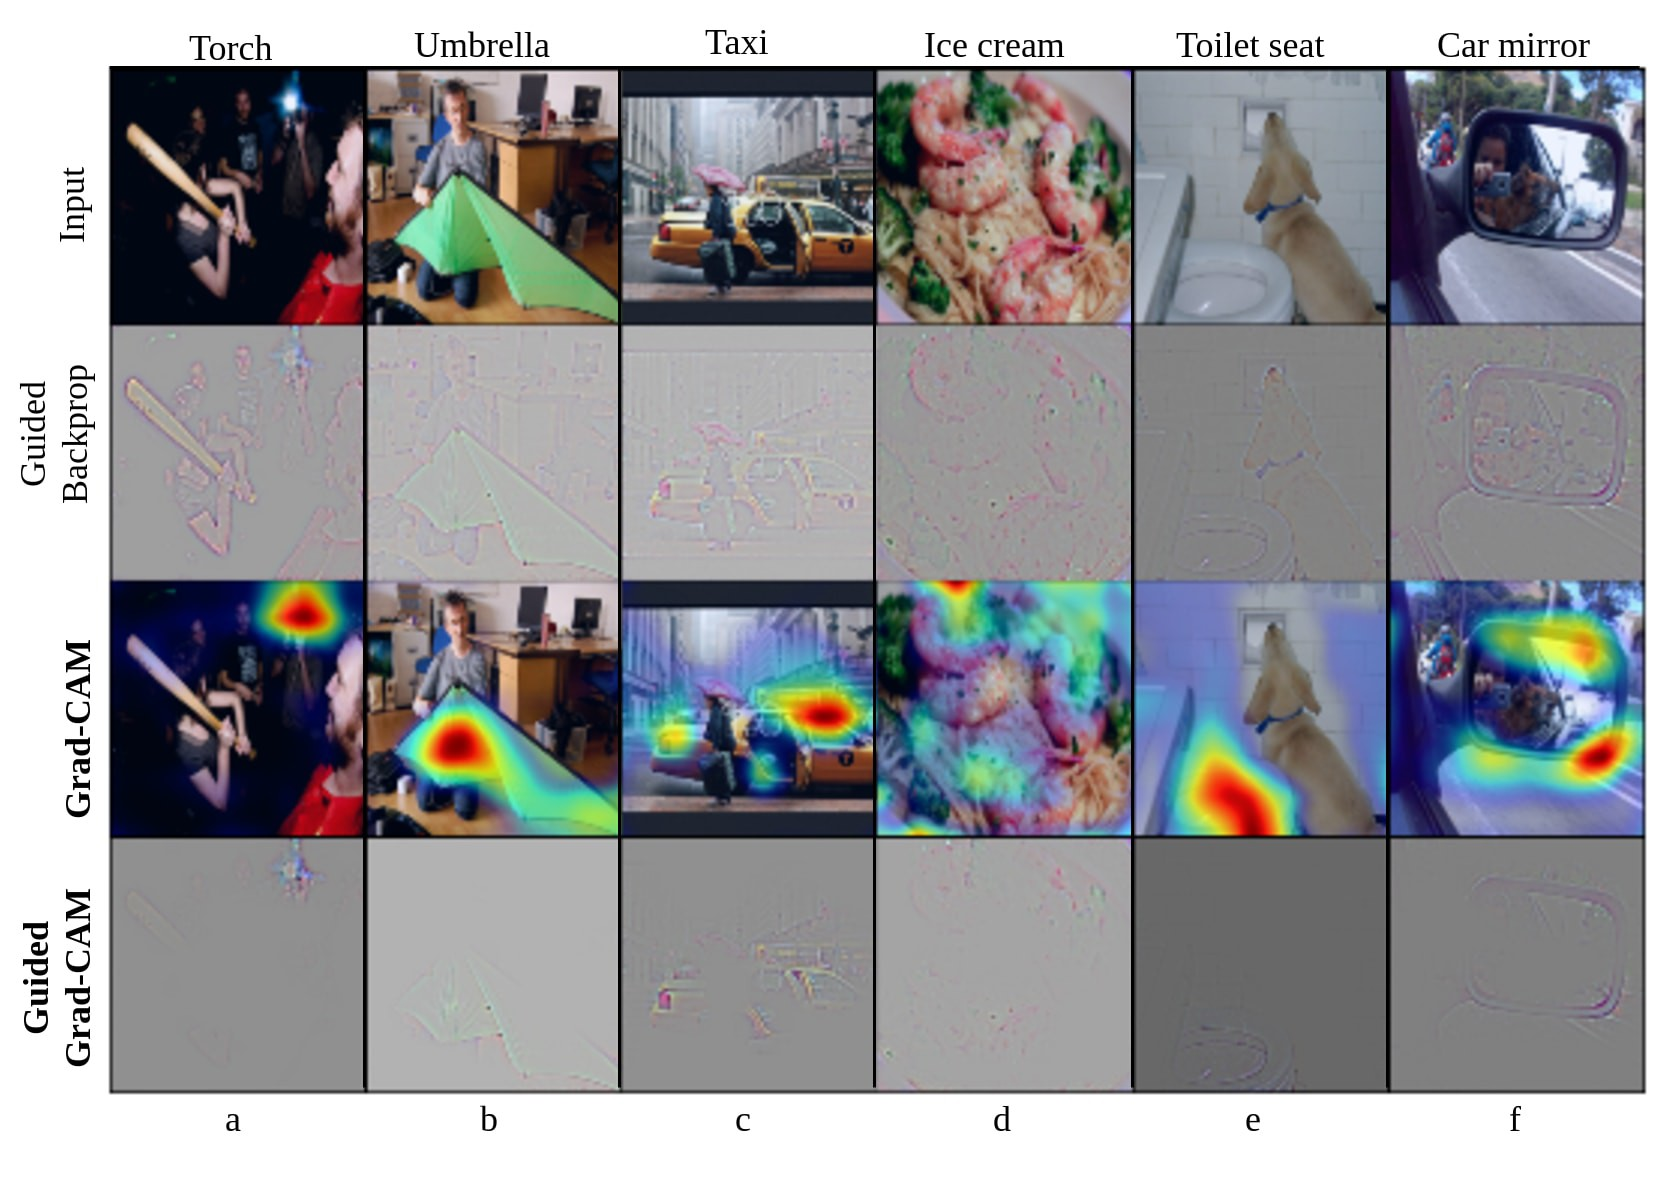
\includegraphics[width=1\linewidth]{figures/classification_supp.jpg}
 \caption{Visualizations for randomly sampled images from the COCO validation dataset.
 Predicted classes are mentioned at the top of each column.}
 \label{fig:classification}
\end{figure*}


We use \gcam{} and \cgb{} to visualize the regions of the image that provide support for a particular prediction.
The results reported in \reffig{fig:classification} correspond to the VGG-16 \cite{simonyan_arxiv14} network trained on ImageNet.


\reffig{fig:classification} shows randomly sampled examples from COCO~\cite{Lin_2014} validation set.
COCO images typically have multiple objects per image and \gcam{} visualizations show precise localization to support the model's prediction.

\cgb{} can even localize tiny objects. For example our approach correctly localizes the predicted class ``torch'' (\reffig{fig:classification}.a) inspite of its size and odd location in the image. Our method is also class-discriminative -- it places attention \emph{only} on the ``toilet seat'' even when a popular ImageNet category ``dog'' exists in the image (\reffig{fig:classification}.e).


We also visualized Grad-CAM, Guided Backpropagation (GB), Deconvolution (DC), GB + \gcam{} (\cgb{}), DC + \gcam{} (\cdec{}) for images from the ILSVRC13 detection val set that have at least 2 unique object categories each.
The visualizations for the mentioned class can be found in the following links.

``computer keyboard, keypad'' class: \\http://i.imgur.com/QMhsRzf.jpg

``sunglasses, dark glasses, shades'' class: \\ http://i.imgur.com/a1C7DGh.jpg

\vspace{-10pt}
\subsection*{2. Image Captioning}

\begin{figure*}
     \centering
     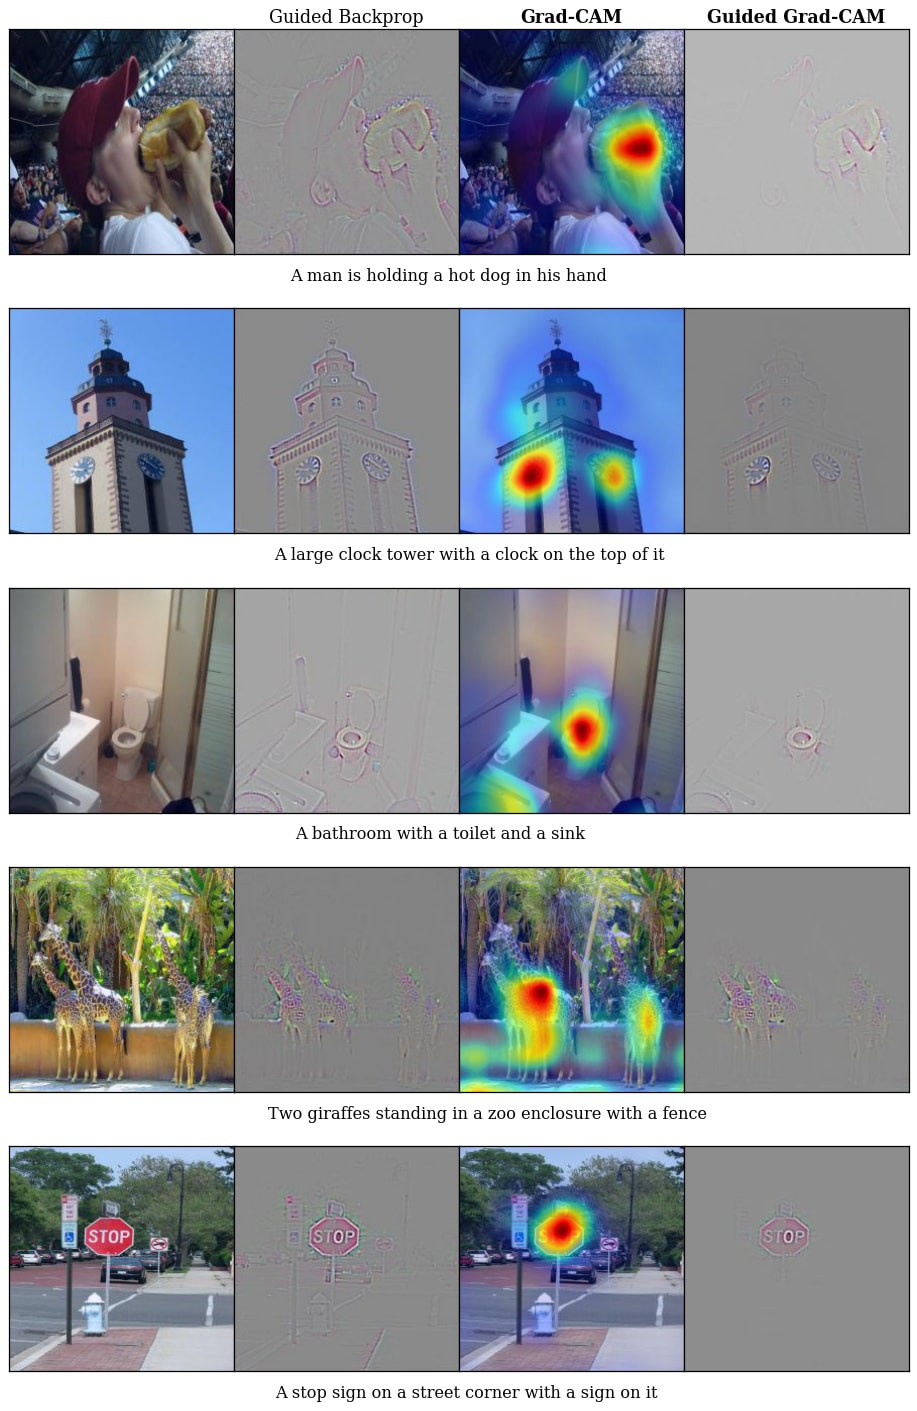
\includegraphics[width=0.83\linewidth]{figures/captioning_supp_new.jpg}
     \caption{\gb{}, \gcam{}  and \cgb{}  visualizations for the captions produced by the Neuraltalk2 image captioning model.}
     \label{fig:sup_captioning}
\end{figure*}

\begin{figure*}
     \centering
     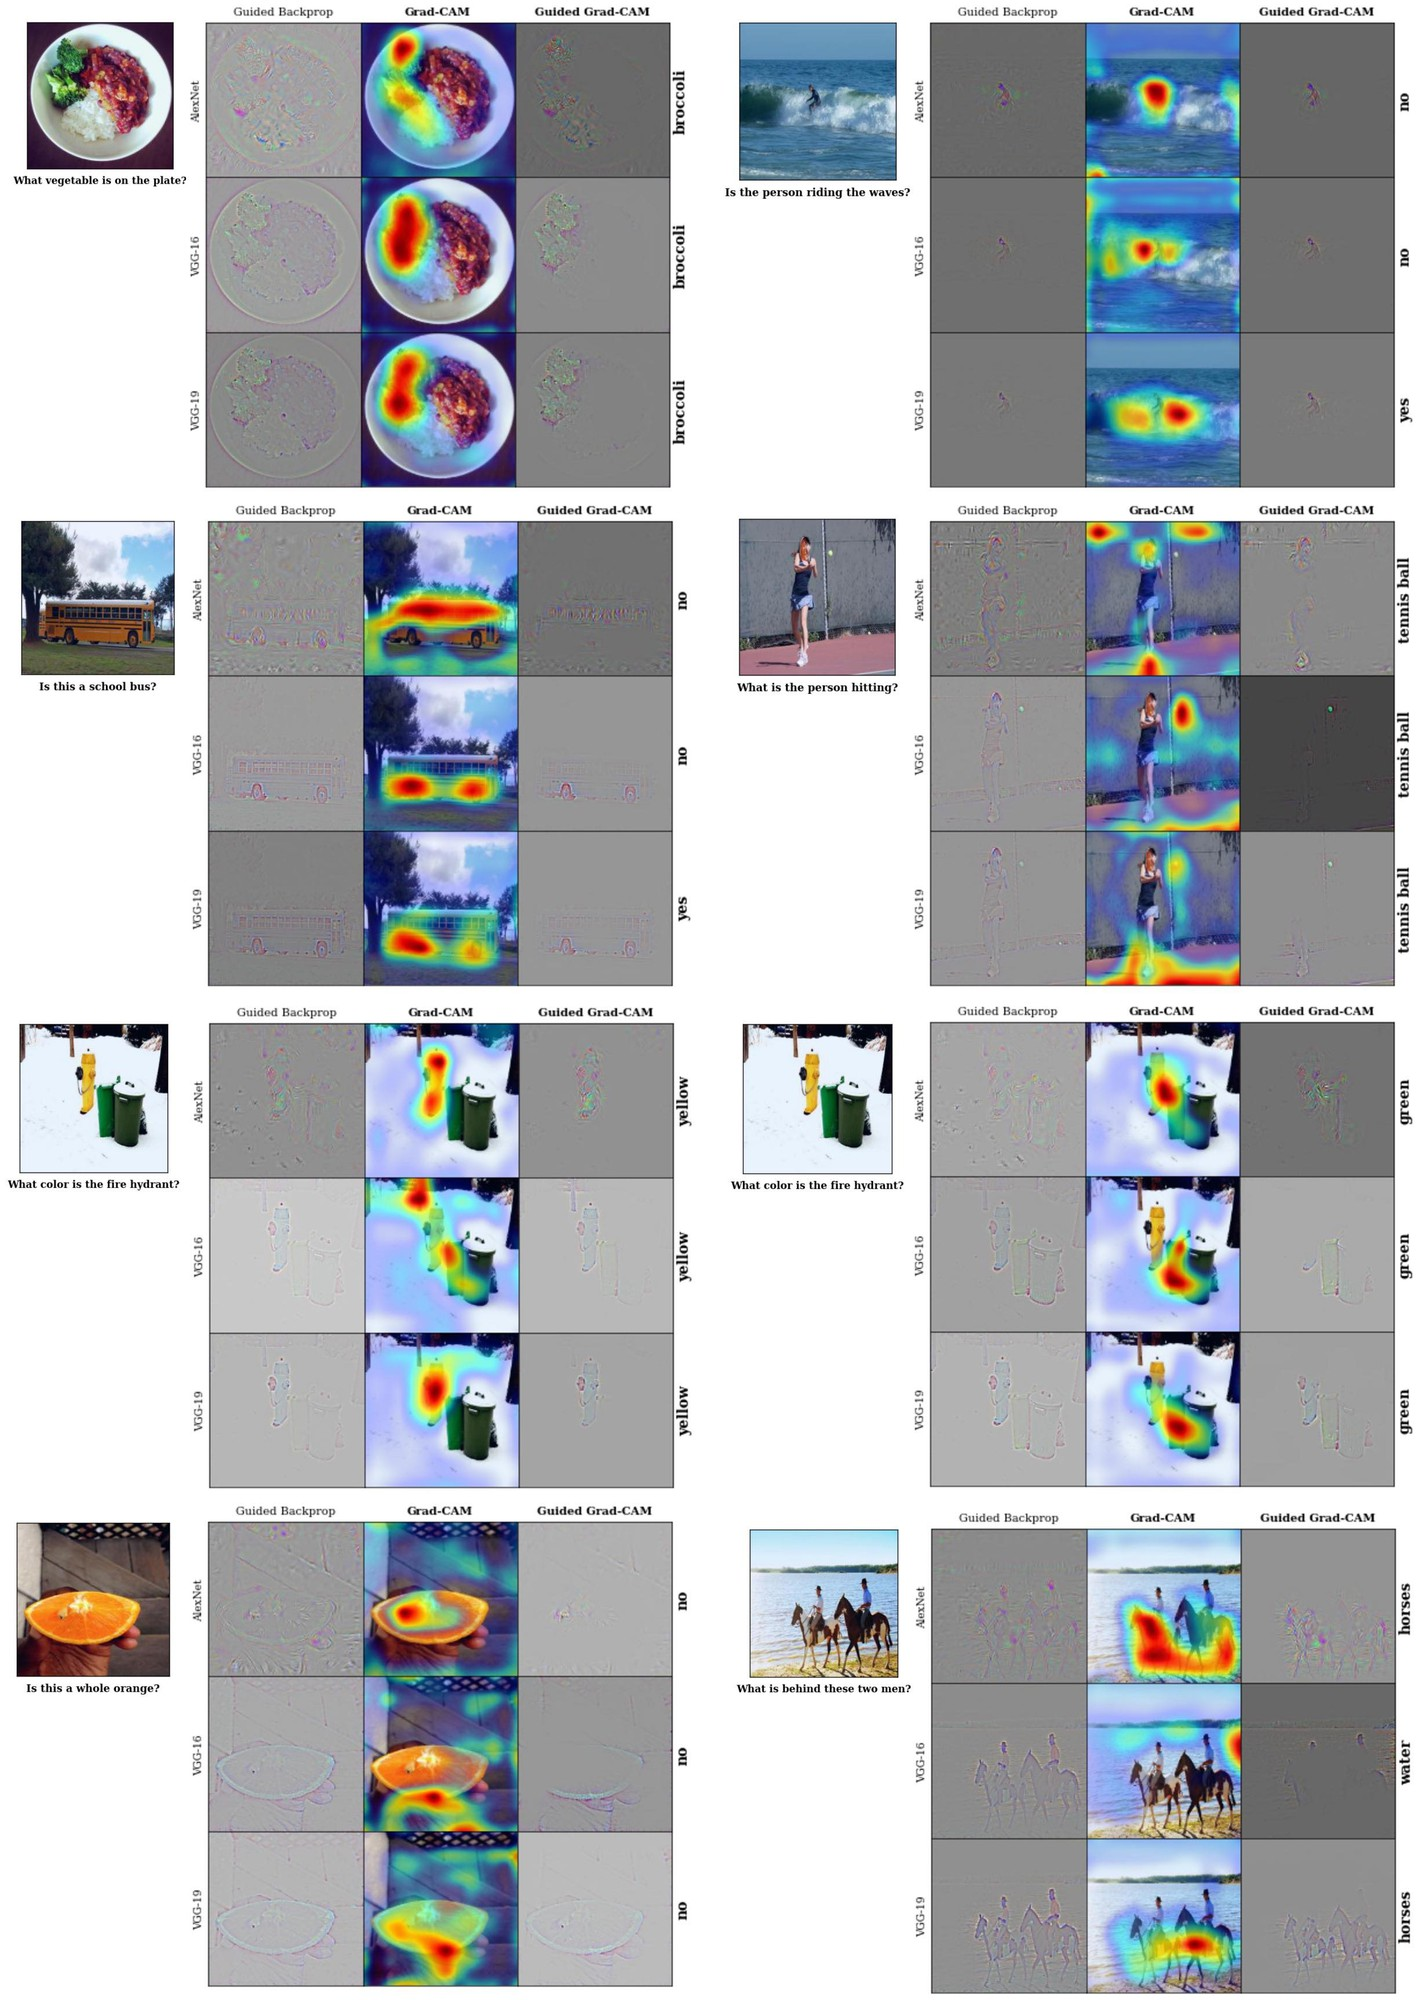
\includegraphics[scale=0.30]{figures/vqa_sup.jpg}
     \caption{\gb{}, \gcam{} and \cgb{}  visualizations for the answers from a VQA model.
     For each image-question pair, we show visualizations for AlexNet, VGG-16 and VGG-19.
     Notice how the attention changes in row 3, as we change the answer from \emph{Yellow} to \emph{Green}.}
     \label{fig:vqa_supp}
\end{figure*}

\begin{figure*}[htp]
 \centering
 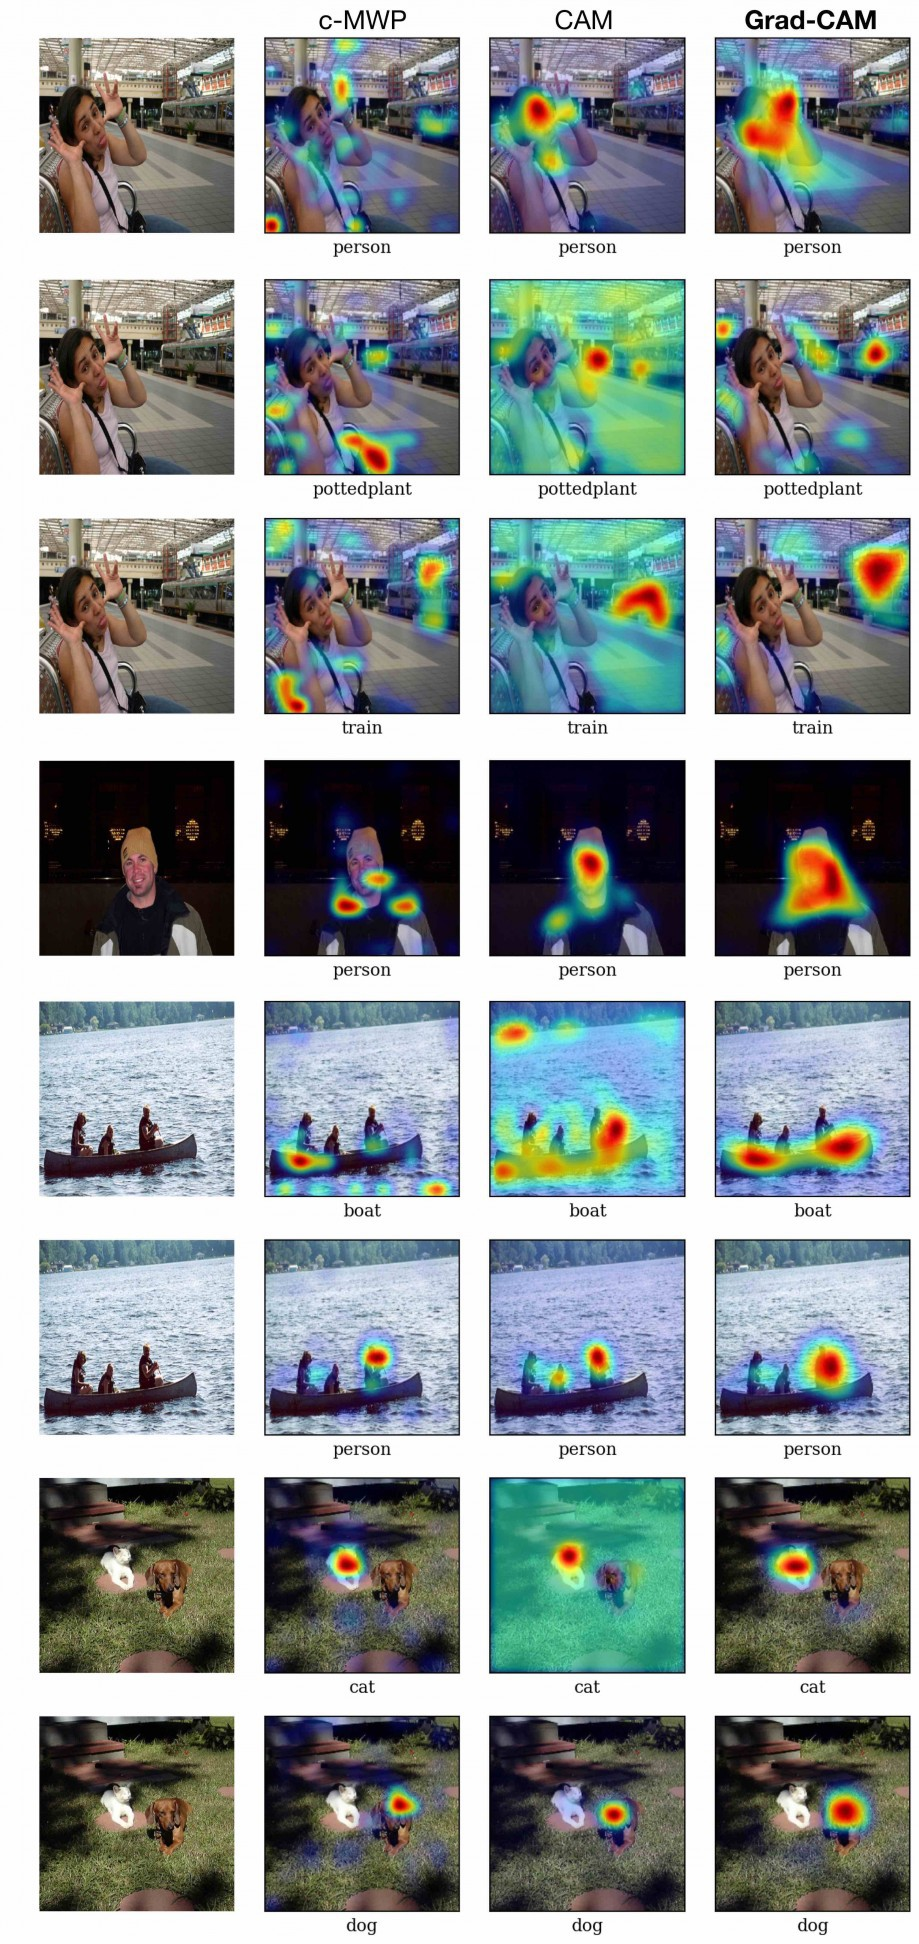
\includegraphics[width=0.65\linewidth]{figures/gcam_pascal.jpg}
 \caption{Visualizations for ground-truth categories (shown below each image) for images sampled from the PASCAL~\cite{pascal-voc-2007} validation set.}
 \label{fig:gcam_pascal}
\end{figure*}


We use the publicly available Neuraltalk2 code and model\footnote{\url{https://github.com/karpathy/neuraltalk2}} for our image captioning experiments.
The model uses VGG-16 to encode the image.
The image representation is passed as input at the first time step to an LSTM that generates a caption for the image.
The model is trained end-to-end along with CNN finetuning using the COCO~\cite{Lin_2014} Captioning dataset.
We feedforward the image to the image captioning model to obtain a caption. \rp{We use \gcam{} to get a coarse localization and combine it with \gb{} to get a high-resolution visualization that highlights regions in the image that provide support for the generated caption.} %


\subsection*{3. Visual Question Answering (VQA)}

\rp{We use \gcam{} and \cgb{} to explain why \rp{a} publicly available VQA model \cite{Lu2015} answered what it answered.}

The VQA model by Lu~\etal uses a standard CNN followed by a fully connected layer to transform the image to 1024-dim to match the \rp{LSTM} embeddings of the question. Then the transformed image and LSTM embeddings are pointwise multiplied to get a combined representation of the image and question and a multi-layer perceptron is trained on top to predict one among 1000 answers.
We show visualizations for the VQA model trained with 3 different CNNs - AlexNet~\cite{krizhevsky_nips12}, VGG-16 and VGG-19~\cite{simonyan_arxiv14}.
Even though the CNNs were not finetuned for the task of VQA, it is interesting to see how our approach can serve as a tool to understand these networks better by providing a localized high-resolution visualization of the regions the model is looking at. Note that these networks were trained with no explicit attention mechanism enforced.

Notice in the first row of \reffig{fig:vqa_supp}, for the question, ``\emph{Is the person riding the waves?}'', the VQA model with AlexNet and VGG-16 answered ``No'', as they concentrated on the person mainly, and not the waves.
On the other hand, VGG-19 correctly answered ``Yes'', and it looked at the regions around the man in order to answer the question.
In the second row, for the question, ``\emph{What is the person hitting?}'', the VQA model trained with AlexNet answered ``Tennis ball'' just based on context without looking at the ball.
Such a model might be risky when employed in real-life scenarios.
It is difficult to determine the trustworthiness of a model just based on the predicted answer.
Our visualizations provide an accurate way to explain the model's predictions and help in determining which model to trust, without making any architectural changes or sacrificing accuracy.
Notice in the last row of \reffig{fig:vqa_supp}, for the question, ``\emph{Is this a whole orange?}'', the model looks for regions around the orange to answer ``No''.

\begin{figure*}[h]
\begin{center}
\begin{subfigure}[t]{\columnwidth}
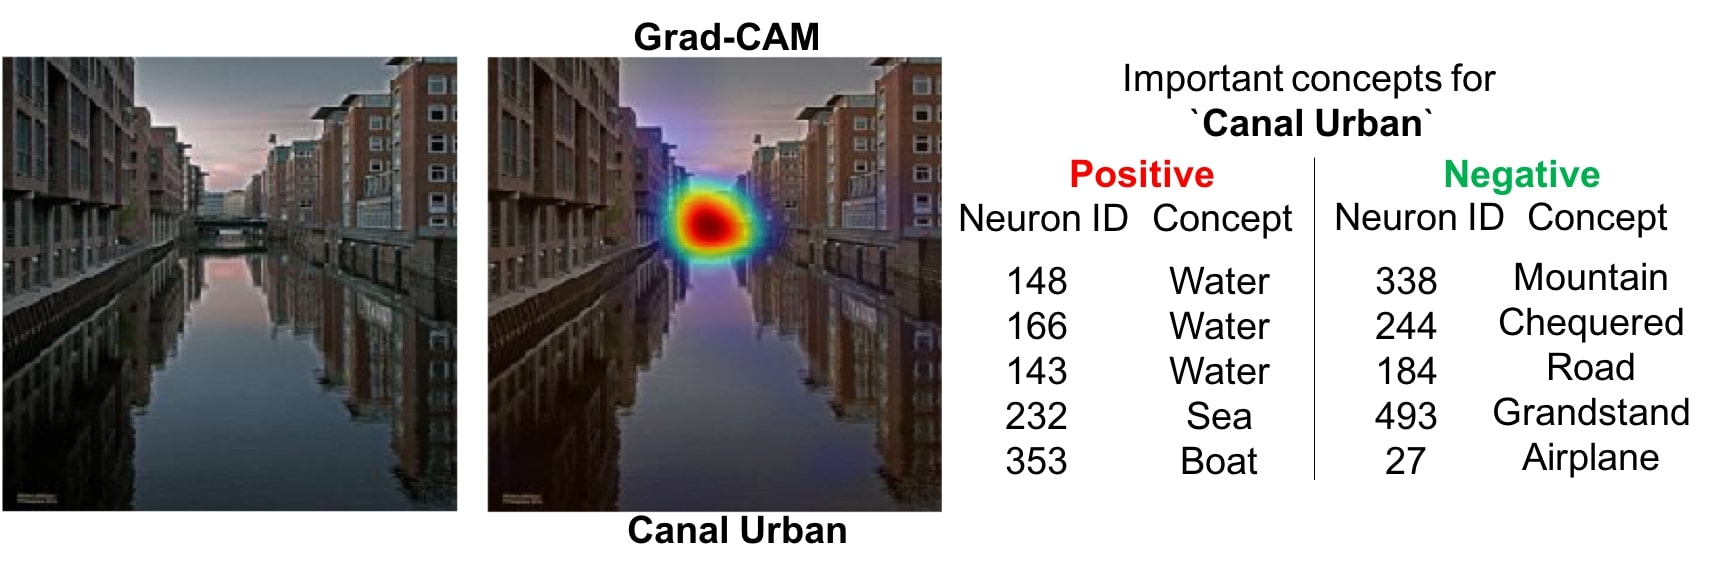
\includegraphics[scale=0.135]{figures/5_pos.jpg}\caption{}
\vspace{10pt}
\end{subfigure}
\begin{subfigure}[t]{\columnwidth}
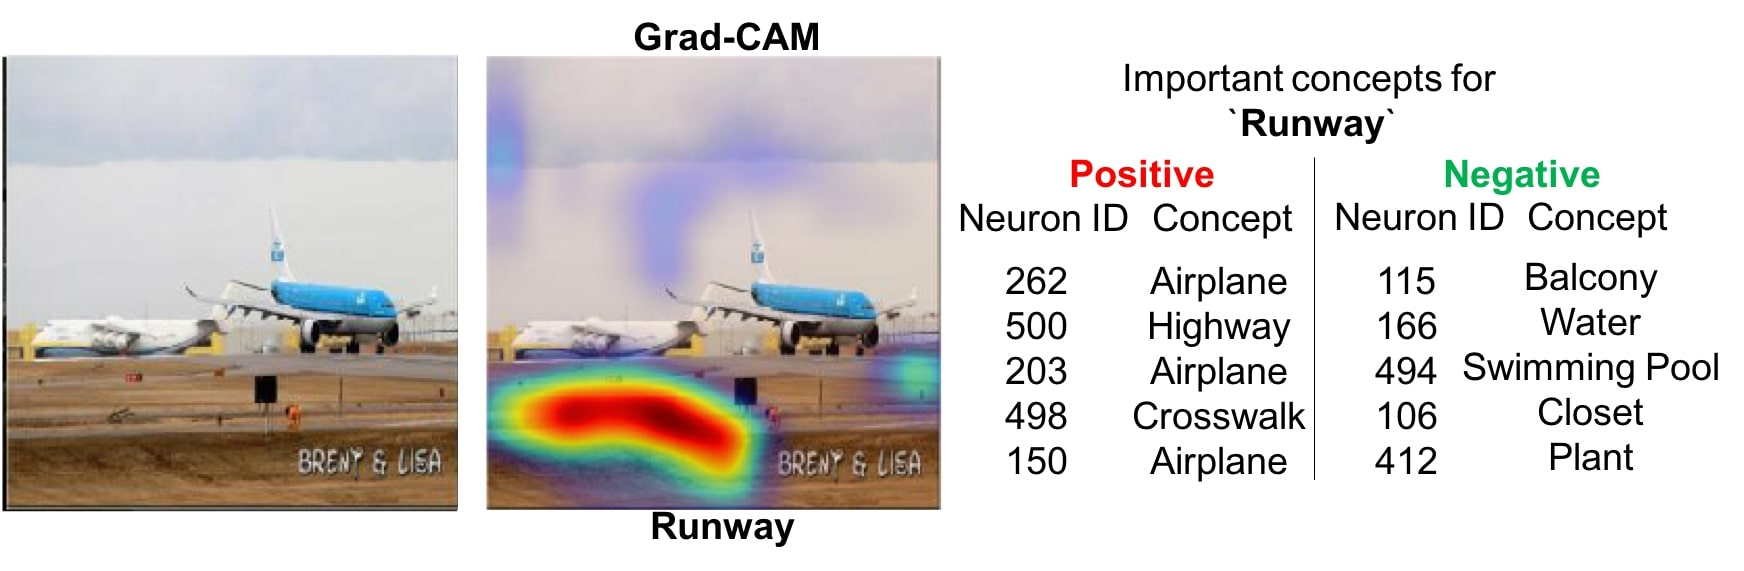
\includegraphics[scale=0.135]{figures/6_pos.jpg}\caption{}
\vspace{10pt}
\end{subfigure}
\begin{subfigure}[t]{\columnwidth}
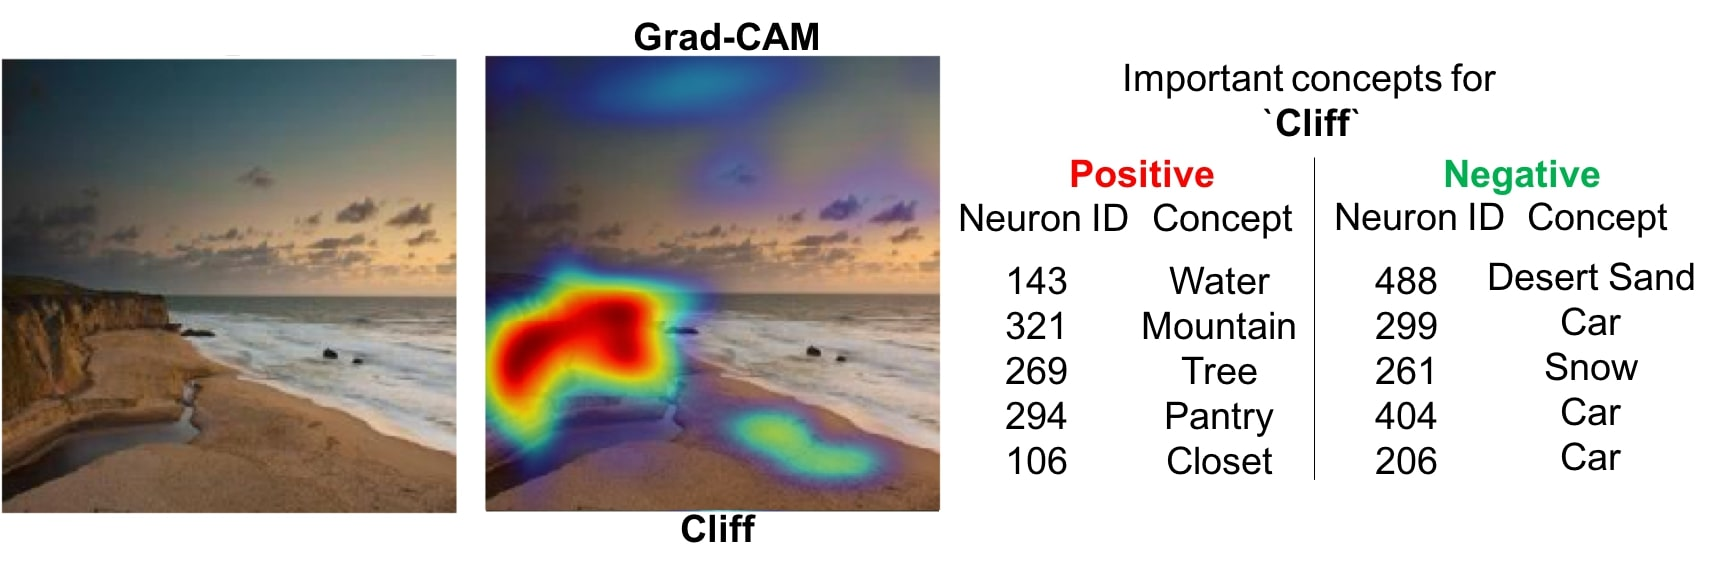
\includegraphics[scale=0.135]{figures/7_pos.jpg}\caption{}
\vspace{10pt}
\end{subfigure}
\begin{subfigure}[t]{\columnwidth}
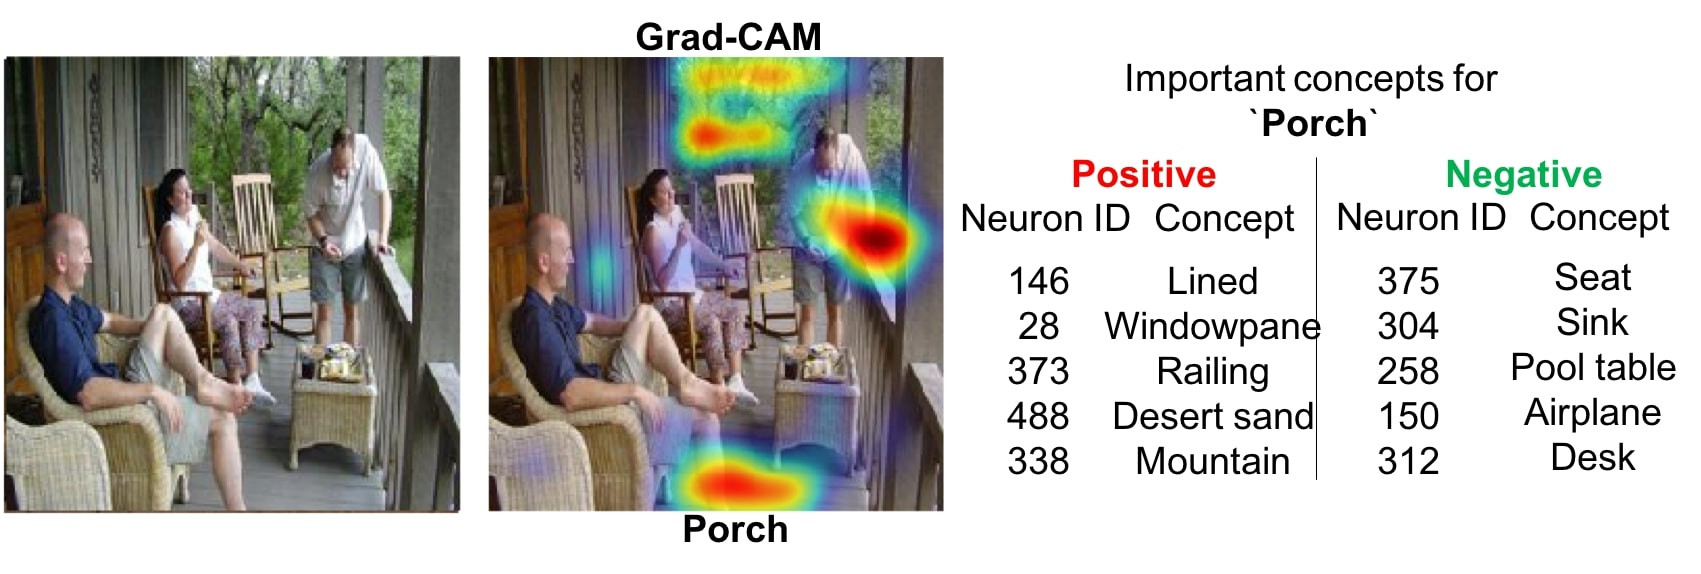
\includegraphics[scale=0.135]{figures/8_pos.jpg}\caption{}
\vspace{10pt}
\end{subfigure}
\begin{subfigure}[t]{\columnwidth}
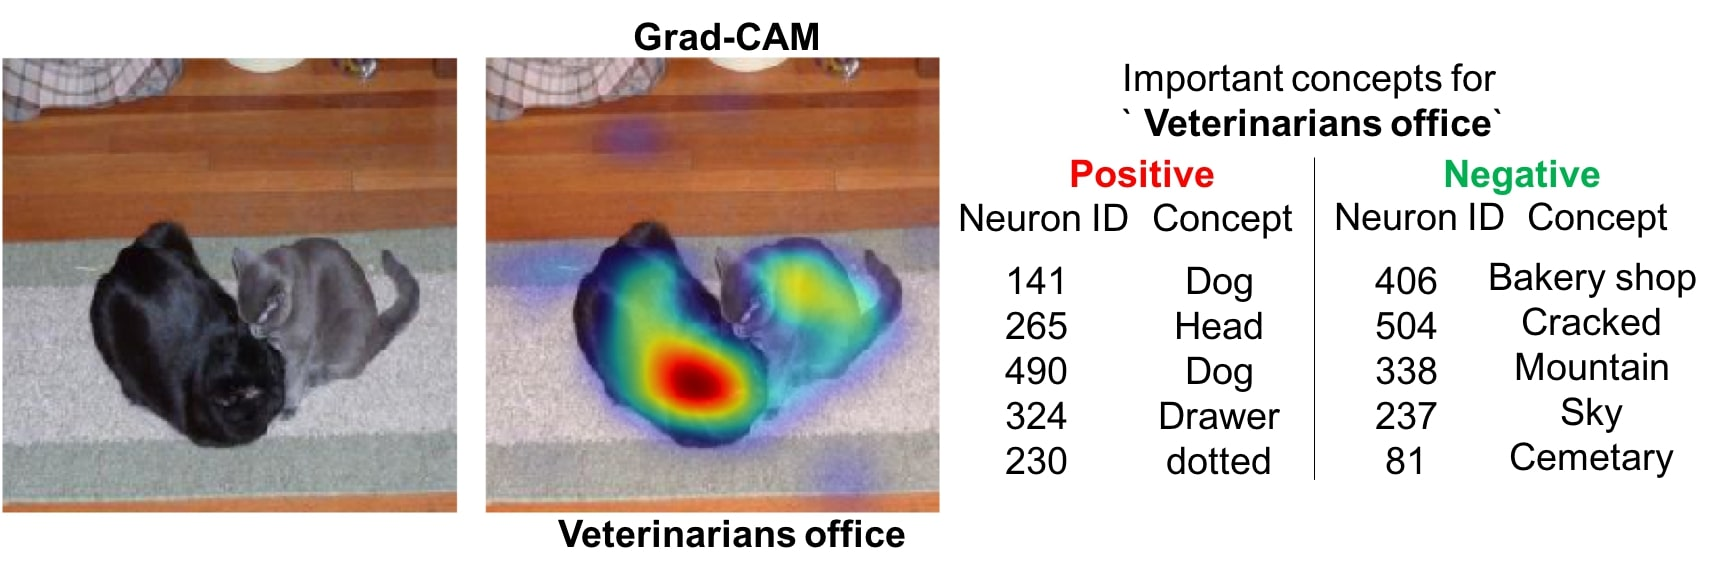
\includegraphics[scale=0.135]{figures/9_pos.jpg}\caption{}
\vspace{10pt}
\end{subfigure}
\begin{subfigure}[t]{\columnwidth}
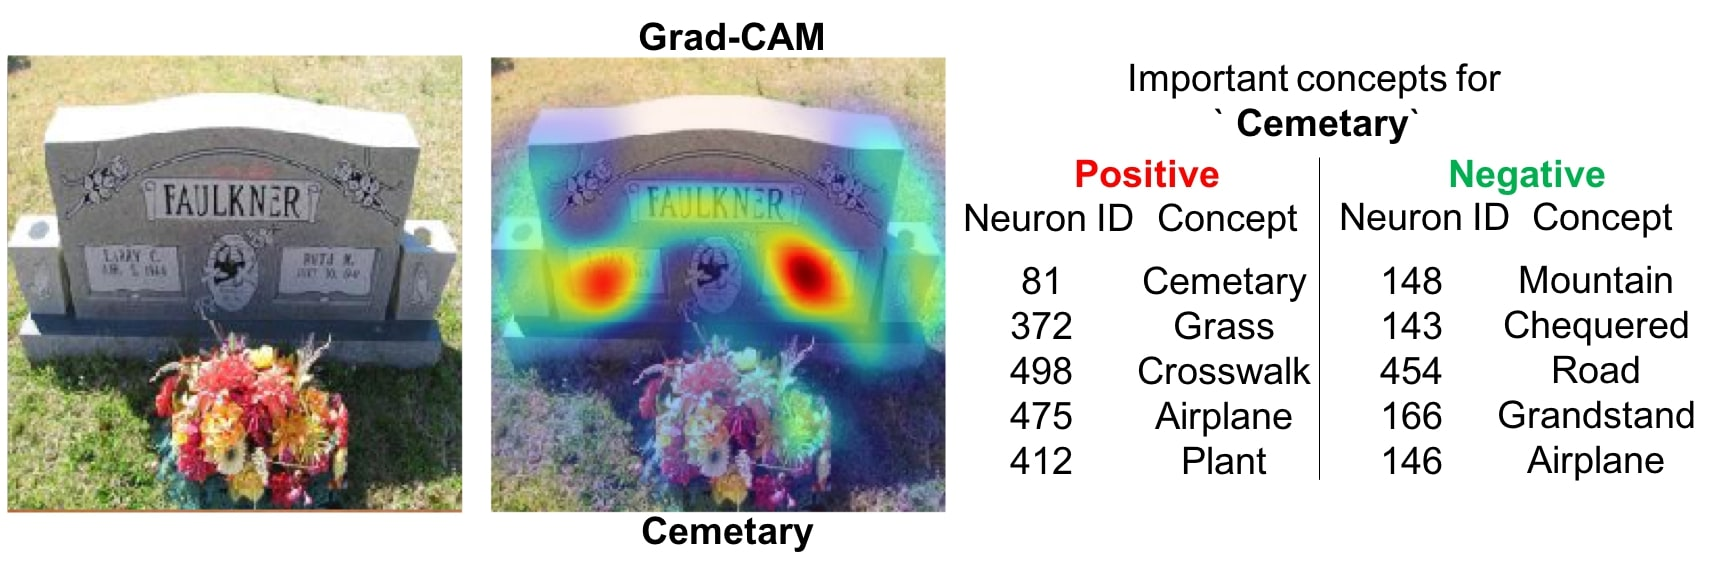
\includegraphics[scale=0.135]{figures/10_pos.jpg}\caption{}
\vspace{10pt}
\end{subfigure}
\begin{subfigure}[t]{\columnwidth}
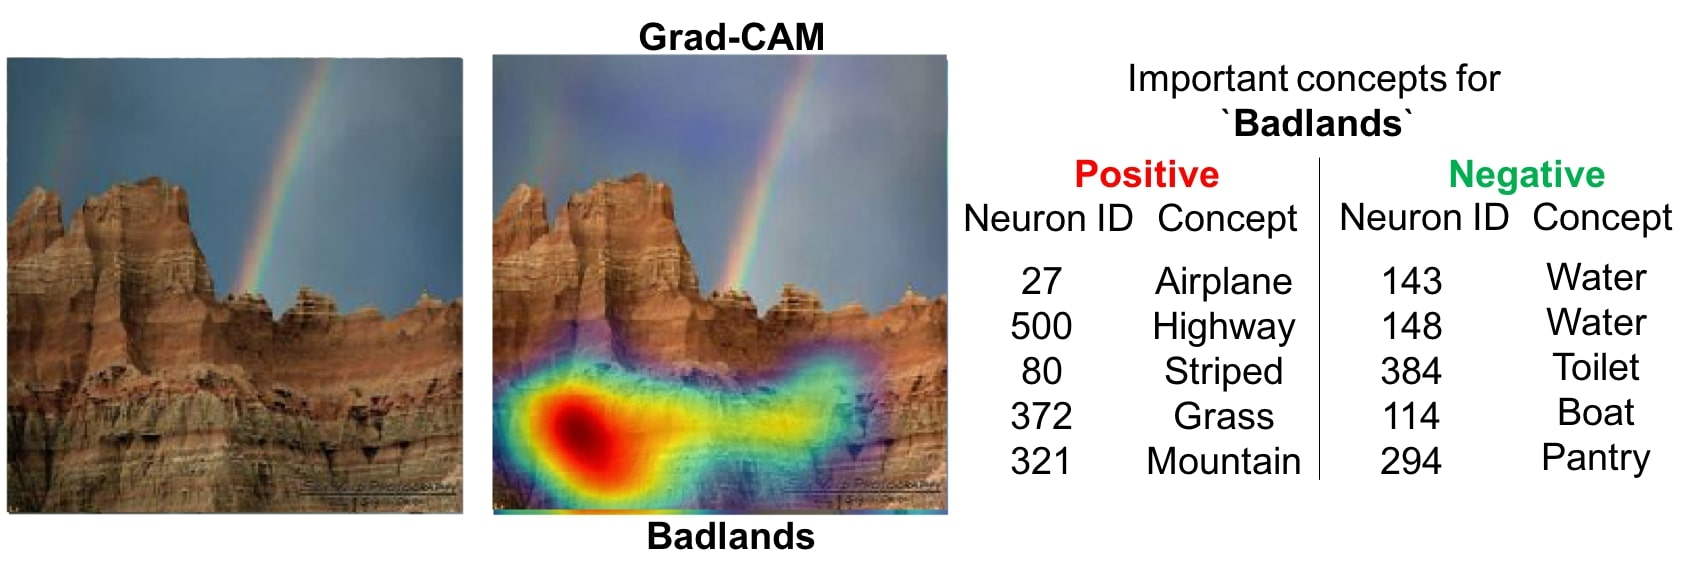
\includegraphics[scale=0.135]{figures/3_neg.jpg}\caption{}
\vspace{10pt}
\end{subfigure}
\begin{subfigure}[t]{\columnwidth}
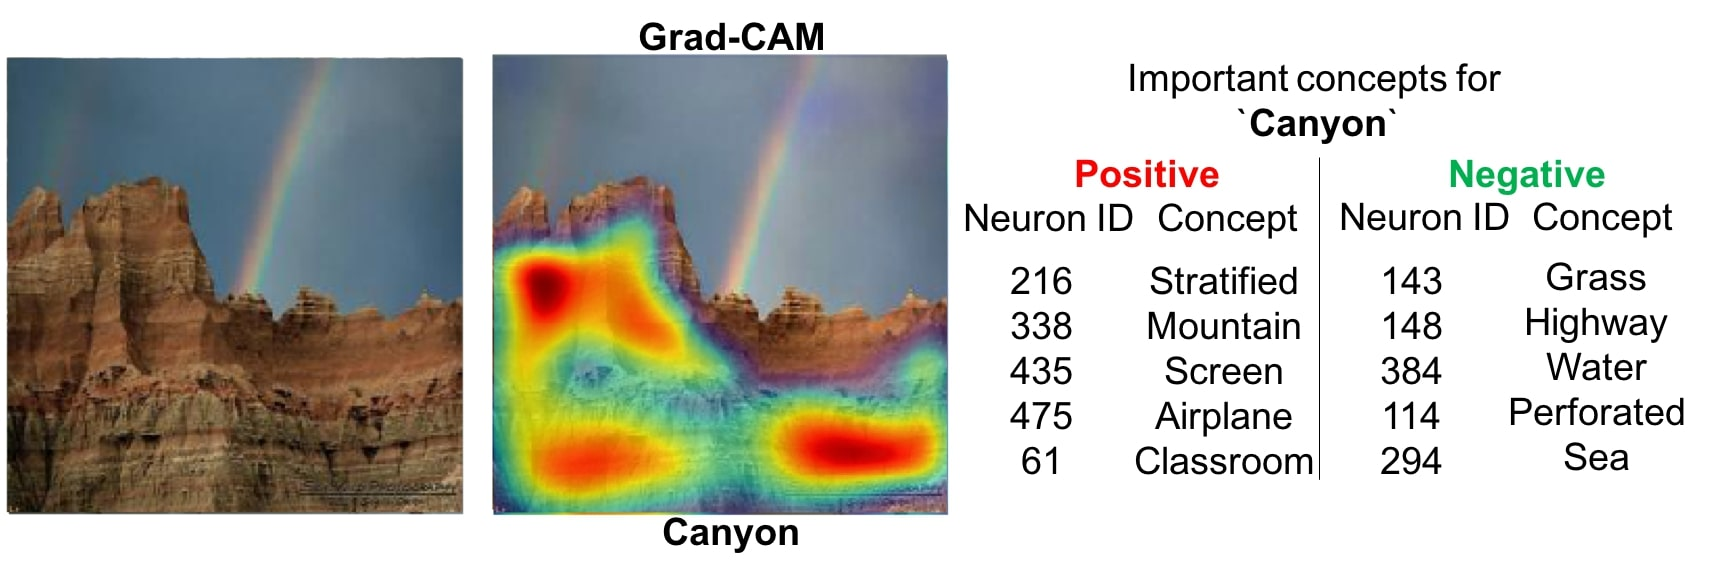
\includegraphics[scale=0.135]{figures/4_neg.jpg}\caption{}
\vspace{10pt}
\end{subfigure}
\begin{subfigure}[t]{\columnwidth}
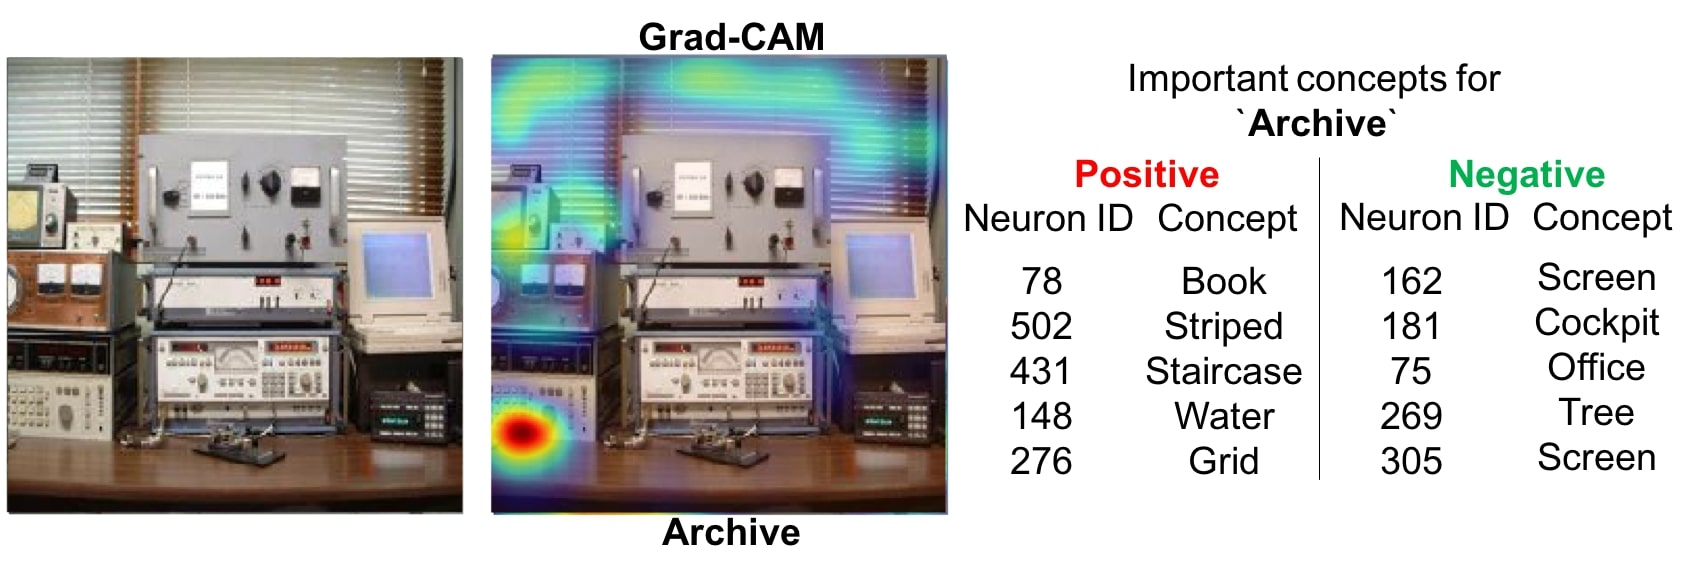
\includegraphics[scale=0.135]{figures/5_neg.jpg}\caption{}
\vspace{10pt}
\end{subfigure}
\begin{subfigure}[t]{\columnwidth}
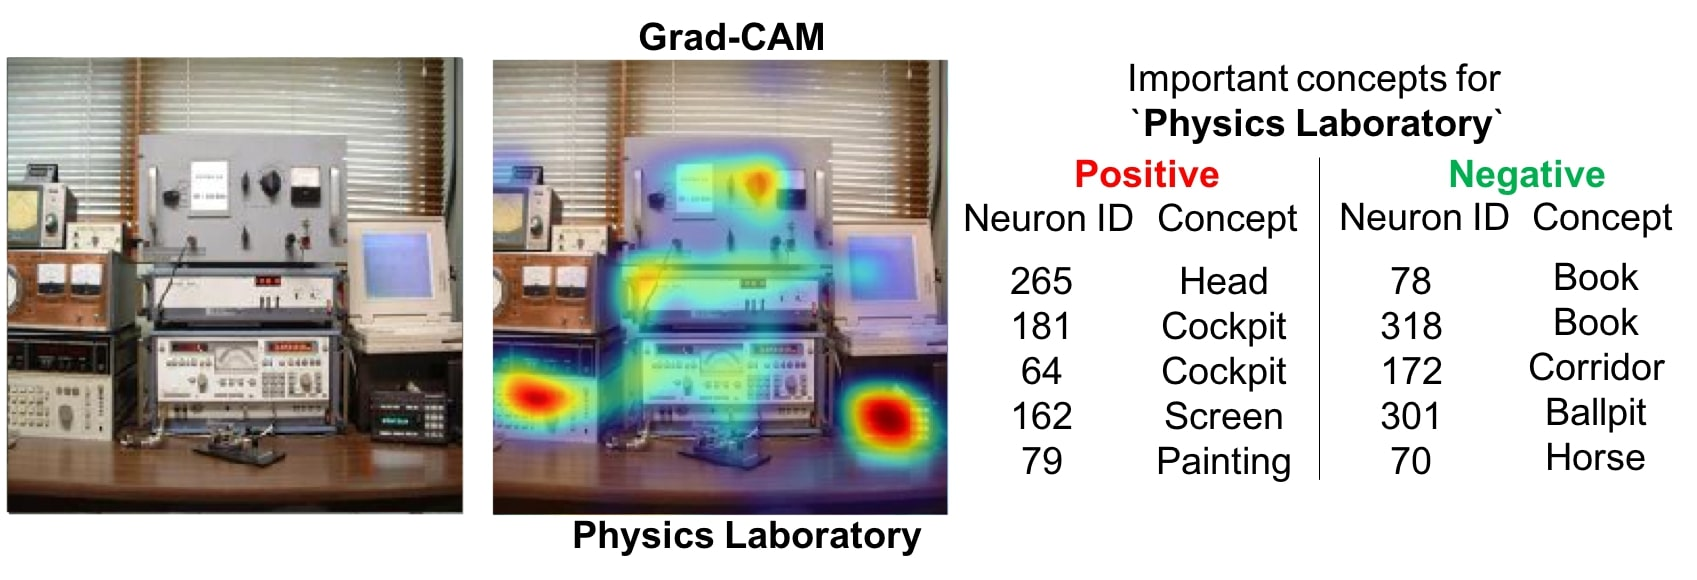
\includegraphics[scale=0.135]{figures/6_neg.jpg}\caption{}
\vspace{10pt}
\end{subfigure}
  \caption{More Qualitative examples showing visual explanations and textual explanations for VGG-16 trained on Places365 dataset (\cite{zhou2017places}). For textual explanations we provide the most important neurons for the predicted class along with their names. Important neurons can be either be persuasive (positively important) or inhibitive (negatively important). 
  The first 3 rows show positive examples, and the last 2 rows show failure cases.}
  \label{fig:sup_text_explanations}
\end{center}
\end{figure*}

